\section{Apresentação Web}
\label{sec:app-web}

Como já mencionado, para a apresentação das informações de captura de maneira
acessível, foi construída uma aplicação Web utilizando as tecnologias
Node.js, MQTT.js, HTML, CSS, Javascript,
Bootstrap e Google Maps API.

Node.js e a biblioteca de cliente MQTT.js foram utilizados para,
da mesma forma exposta no \autoref{code-mqttjs-client}, conectar
uma aplicação escrita em Javascript com o \emph{MQTT Broker}. Esta
aplicação recupera as informações sobre os dispositos descobertos e as
classifica por proximidade de cada sensor para compor a lista de dispositios
por sensor vista no lado direito da \autoref{fig-web-app}.

Já o HTML, CSS, Javascript e Bootstrap foram
utilizados para estruturar, estilizar, inflar e animar as informações. Em
especial, o Bootstrap forneceu a estrutura de cabeçalho, rodapé e colunas,
além do esquema de cores.

A Google Maps API juntamente com um pouco de CSS e
Javascript fornece o mapa visto no lado direito da \autoref{fig-web-app}.
Nele estão reprensentadas as localizações geográficas de cada sensor
representados pelos marcadores nas cores azul e verde.

\begin{figure}[htb]
	\caption{\label{fig-web-app}Web APP}
	\begin{center}
		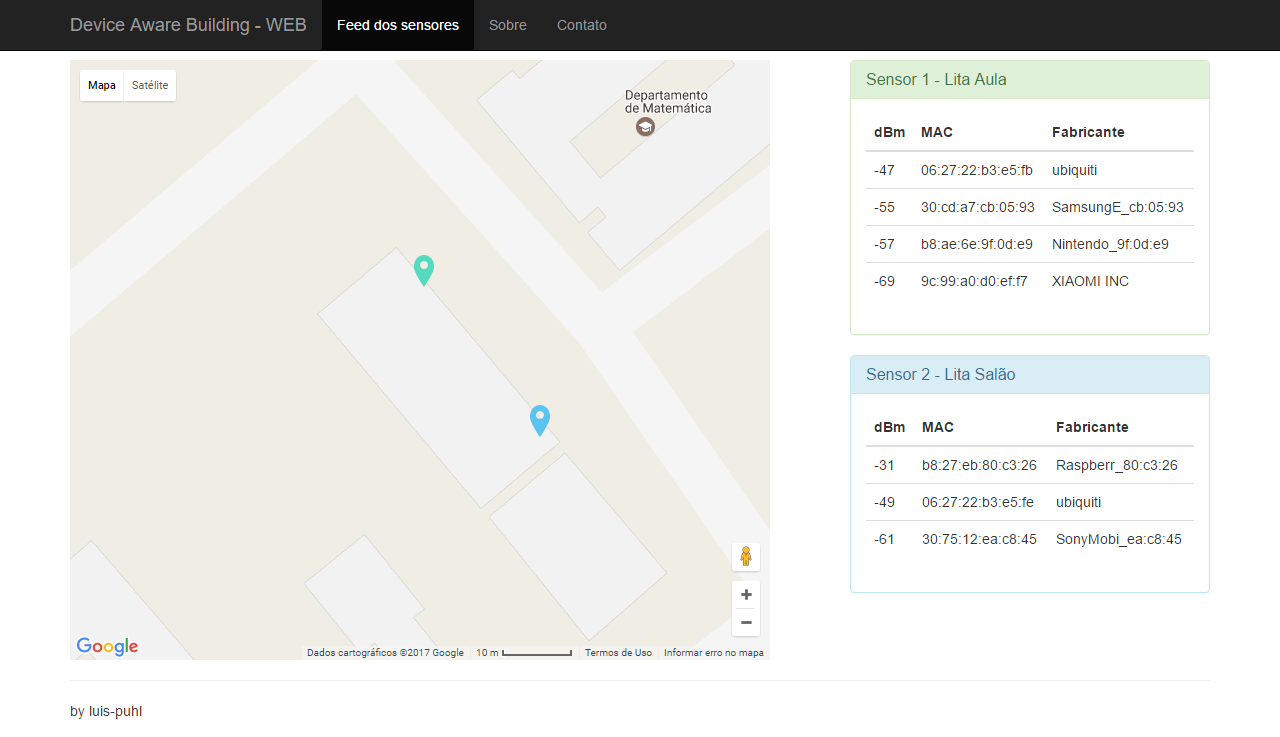
\includegraphics[width=1\textwidth]{053-web/web-app.png}
	\end{center}
	\legend{Fonte: Elaborada pelo autor}
\end{figure}
